\documentclass{beamer}
\usepackage{graphicx}
\usepackage{graphics}
\usepackage{hyperref}
\usepackage[english]{babel}
\usepackage[T1]{fontenc}
\usepackage[utf8]{inputenc}
\usepackage{xfrac}


\mode<presentation>
{
    \usetheme{AMUFree-kk}
    \setbeamercovered{transparent = 28}
}
\title{World of Transformer}
\date{2019}
\author{Karol Kaczmarek}
\setbeamertemplate{bibliography item}{[\theenumiv]}


\begin{document}

\begin{frame}
    \titlepage
\end{frame}

\iffalse
\AtBeginSection[]
{
    \begin{frame}
        \frametitle{Outline}
        \tableofcontents[currentsection]
    \end{frame}
}
\fi




% Transformer
\section{Transformer}
\begin{frame}
    \frametitle{Transformer \cite{transformer}}
    \begin{itemize}
        \item June 2017
        \item encoder-decoder model
        \item dispensing with recurrence and convolutions entirely
        \item attention mechanism (MultiHeadAttention)
        \item positional encoding
    \end{itemize}
\end{frame}

\begin{frame}
    \frametitle{Architecture}
    \begin{center}
        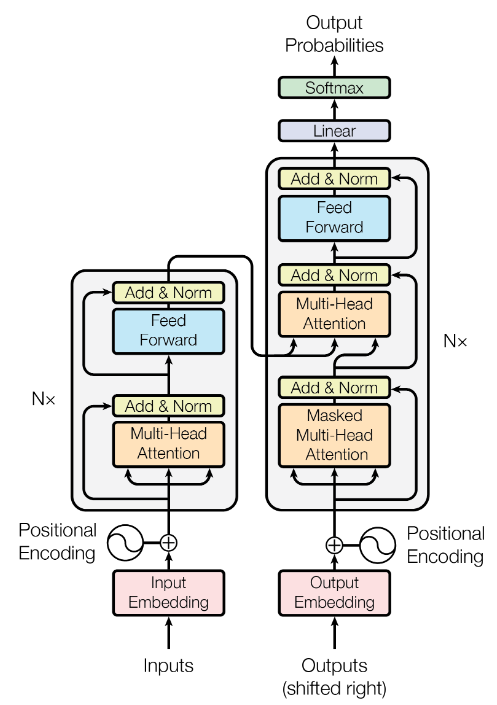
\includegraphics[scale=1.15]{img/transformer.png}
    \end{center}
\end{frame}

\begin{frame}
    \frametitle{Multi-head attention}
    \begin{center}
        $ Attention (Q, K, V) = softmax(\frac{QK^T}{\sqrt{d_k}})V $ \\
        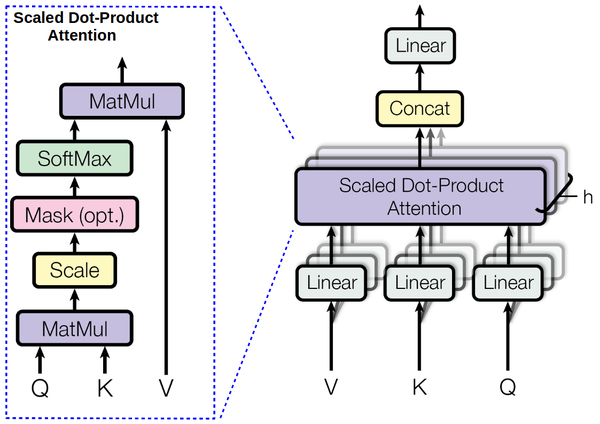
\includegraphics[scale=0.45]{img/multi_head_attention.png}
    \end{center}
\end{frame}



% GPT2
\section{OpenAI GPT-2}
\begin{frame}
    \frametitle{GPT-2 \cite{gpt2}}
    \begin{itemize}
        \item February 2019
        \item based on Transformer \cite{transformer} (GPT-1)
        \item Byte Pair Encoding (BPE) \cite{bpe} on the byte level
        \begin{itemize}
        	\item $<$UNK$>$ occurs 26 times in 40 billion bytes
        \end{itemize}
        \item use custom regex text splitter
        \item trained on 40GB of text collected from the Internet (WebText)
        \begin{itemize}
        	\item it's not Common Crawl (quality issues)
        	\item OpenWebText as an alternative
        \end{itemize}
        \item GELU -- Gaussian Error Linear Unit \cite{gelu}
    \end{itemize}
\end{frame}

\begin{frame}
    \frametitle{Models}
    \begin{center}
    	\begin{tabular}{ l | l | c | c}
    		$Name$ & $Parameters$ & $Layers$ & $d_{model}$ \\
    		\hline
    		Base & $117M$ & $12$ & $768$ \\
    		Medium & $345M$ & $24$ & $1024$ \\
    		Large & $762M$ & $36$ & $1280$ \\
    		XL & $1542M$ & $48$ & $1600$ \\
    	\end{tabular}
    \end{center}
\end{frame}

\begin{frame}
    \frametitle{GELU -- Gaussian Error Linear Unit \cite{gelu}}
    \begin{center}
        GELU - $ sigmoid(1.702 \cdot x) \cdot x $ \\
        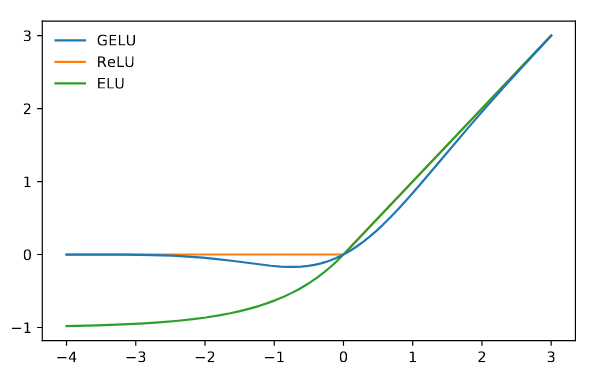
\includegraphics[scale=2.0]{img/gelu.png}
    \end{center}
\end{frame}

\begin{frame}
    \frametitle{Comparing different levels of BPE}
    \begin{center}
    	\begin{tabular}{l | l | l}
    		& \textbf{BPE based on bytes} & \textbf{BPE based on characters} \\
    		\hline
    		1 & 'I like cats.' & 'I like cats.' \\
    		\hline
    		2 & 'I', ' like', 'cats', '.' & 'I', 'like', 'cats', '.' \\
    		\hline
    		3 & $[$'0x49'$]$, & -- \\
    		& $[$'0x20', '0x6c', '0x69', & \\
    		& '0x6b', '0x65'$]$, & \\
    		& $[$'0x20', '0x63', '0x61', & \\
    		& '0x74', '0x73'$]$, & \\
    		& $[$'0x2e'$]$ & \\
    		\hline
    		4 & 'I', 'Ġlike', 'Ġcats', '.' & -- \\
    		\hline
    		5 & 'I', 'Ġli@@', 'ke', & 'I', 'li@@', 'ke' \\
    		& 'Ġca@@', 'ts', '.' & 'ca@@', 'ts', '.' \\
    	\end{tabular}
    \end{center}
\end{frame}

\begin{frame}
    \frametitle{Comparing different levels of BPE}
    \begin{center}
    	\begin{tabular}{l | l | l}
    		& \textbf{BPE based on bytes} & \textbf{BPE based on characters} \\
    		\hline
    		1 & 'Zażółć gęślą jaźń.' & 'Zażółć gęślą jaźń.' \\
    		\hline
    		2 & 'Zażółć', ' gęślą', ' jaźń', '.' & 'Zażółć', 'gęślą', 'jaźń', '.' \\
    		\hline
    		4 & 'ZaÅ\sfrac{1}{4}óÅĤÄĩ', 'ĠgÄĻÅĽlÄh', & -- \\
    		  &  'ĠjaźÅH', '.' & \\
    		\hline
    		5 & 'Z@@' 'a@@' 'Å@@' '\sfrac{1}{4}@@''  & 'Z@@' 'a@@' 'ż@@' \\
    		  & 'ó@@' 'ÅĤ@@' 'Äĩ' & 'ó@@' 'ł@@' 'ć' \\
    		  & 'Ġg@@' 'Ä@@' 'Ļ@@' 'Å@@' & 'g@@' 'ę@@' 'ś@@' \\
    		  & 'Ľ@@' 'l@@' 'Ä@@' 'h' & 'l@@' 'ą' 'j@@' \\
    		  & 'Ġja@@' 'Å@@' 'º@@' 'Å@@' & 'a@@' 'ź@@' 'ń' '.' \\
    		  &  'H' '.' & \\
    	\end{tabular}
    \end{center}
\end{frame}



% BERT
\section{BERT}
\begin{frame}
    \frametitle{BERT \cite{bert}}
    \begin{itemize}
        \item \textbf{BERT} -- \textbf{B}idirectional \textbf{E}ncoder \textbf{R}epresentations from \textbf{T}ransformers = bidirectional Transformers
    \end{itemize}
    \begin{center}
        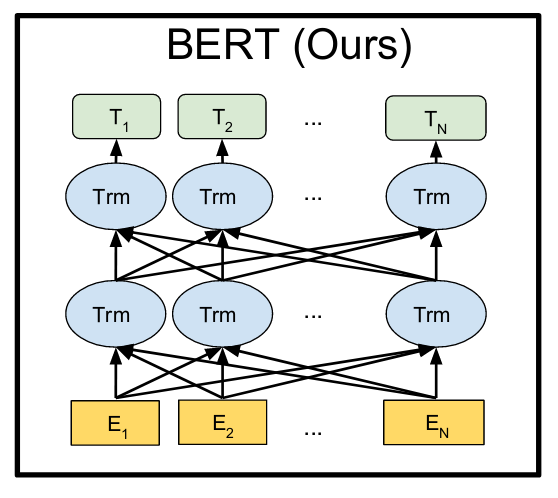
\includegraphics[scale=1.0]{img/bert.png}
    \end{center}
\end{frame}

\begin{frame}
    \frametitle{BERT input representation}
    \begin{itemize}
        \item \textbf{[CLS]} -- the special classification embedding
        \item \textbf{[SEP]} -- the sentences separator, sentence pairs are packed together into a single sequence
        \item segment embeddings
    \end{itemize}
    \begin{center}
        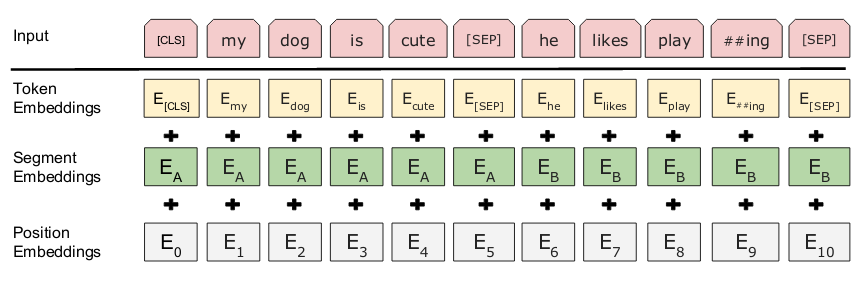
\includegraphics[scale=1.4]{img/bert_input.png}
    \end{center}
\end{frame}

\begin{frame}
    \frametitle{Masked Language Model (MLM)}
    \begin{itemize}
        \item masking some percentage of the input tokens at random
        \item predicting only those masked tokens (\textbf{[MASK]})
        \item mask 15\% of all
        \item masking procedure:
        \begin{itemize}
        	\item 80\% of the time - replace the word with the \textbf{[MASK]} token
        	\begin{itemize}
        		\item \textit{my dog is hairy $\rightarrow$ my dog is [MASK]}
        	\end{itemize}
        	\item 10\% of the time - replace the word with a random word
        	\begin{itemize}
        		\item \textit{my dog is hairy $\rightarrow$ my dog is apple}
        	\end{itemize}
        	\item 10\% of the time - keep the word  unchanged
        	\begin{itemize}
        		\item \textit{my dog is hairy $\rightarrow$ my dog is hairy}
        	\end{itemize}
        \end{itemize}
    \end{itemize}
\end{frame}



% PyTorch
\section{PyTorch}
\begin{frame}
    \frametitle{PyTorch}
    \begin{itemize}
        \item PyTorch 1.2 support Transformer architecture:
        \begin{itemize}
            \item nn.Transformer
            \item nn.TransformerEncoder
            \item nn.TransformerEncoderLayer
            \item nn.TransformerDecoder
            \item nn.TransformerDecoderLayer
            \item nn.MultiheadAttention
        \end{itemize}
        \item PyTorch 1.3 current version
    \end{itemize}
\end{frame}



% Evolved Transformer
\section{Evolved Transformer}
\begin{frame}
    \frametitle{Evolved Transformer \cite{evolved}}
    \begin{itemize}
        \item January/February 2019
        \item $7,30 \cdot 10^{115}$ possible models
        \begin{itemize}
            \item use fraction of data (WMT'14 En-De)
            \item aggressive early stopping (allows models that are consistently performing well to train for more steps)
        \end{itemize}
        \item Depth-wise separable convolutions (Xception\cite{xception})
        \item Gated Linear Units
        \item Swish activation
    \end{itemize}
\end{frame}

\begin{frame}
    \frametitle{Evolved Transformer Encoder}
    \begin{center}
        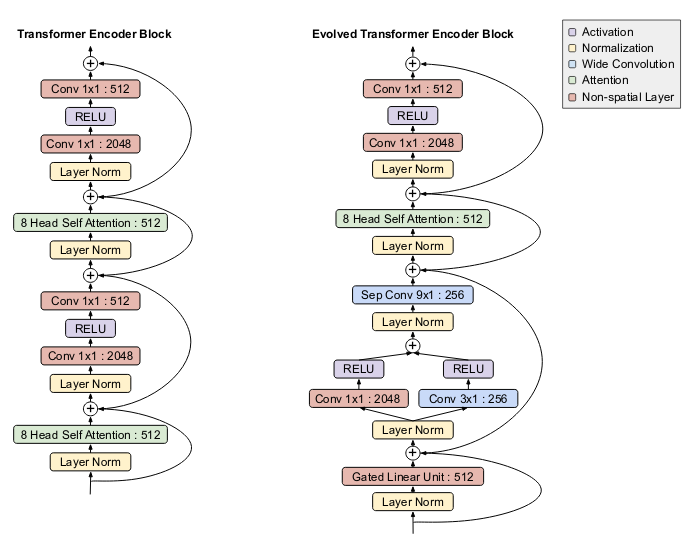
\includegraphics[scale=1.5]{img/evolved-transformer-encoder.png}
    \end{center}
\end{frame}

\begin{frame}
    \frametitle{Evolved Transformer Decoder}
    \begin{center}
        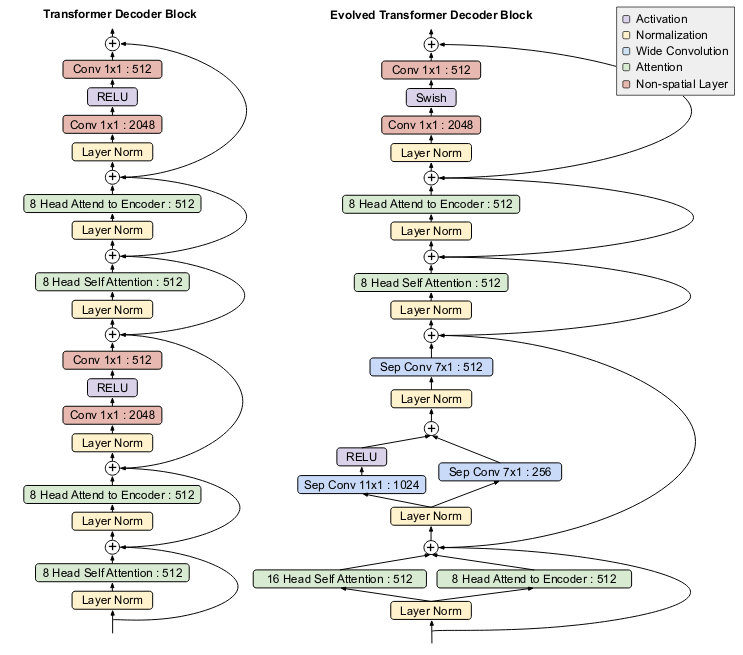
\includegraphics[scale=1.25]{img/evolved-transformer-decoder.png}
    \end{center}
\end{frame}

\begin{frame}
    \frametitle{Score}
    \begin{center}
        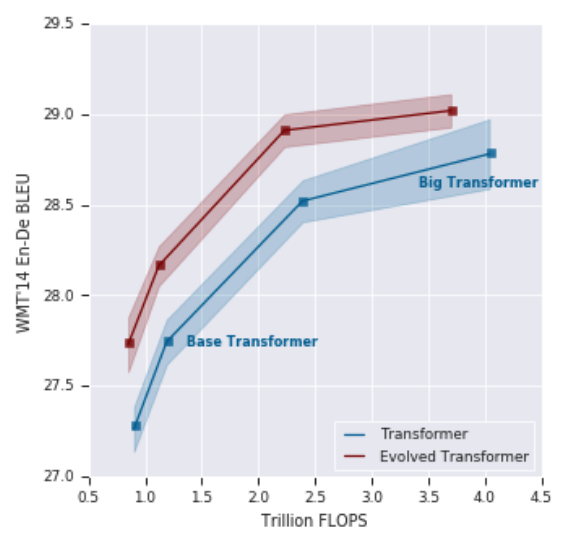
\includegraphics[scale=1.5]{img/evolved-transformer-score.png}
    \end{center}
\end{frame}



% XLM
\section{XLM}
\begin{frame}
    \frametitle{XLM \cite{xlm}}
    \begin{itemize}
        \item January 2019
        \item created by Facebook
        \item based on BERT
        \item use text streams of an arbitrary number of sentences instead of pairs of sentences
        \item no next sentence prediction
        \item 12 layers (BERT - 24 layers)
    \end{itemize}
\end{frame}

\begin{frame}
    \frametitle{XLM}
    \begin{center}
        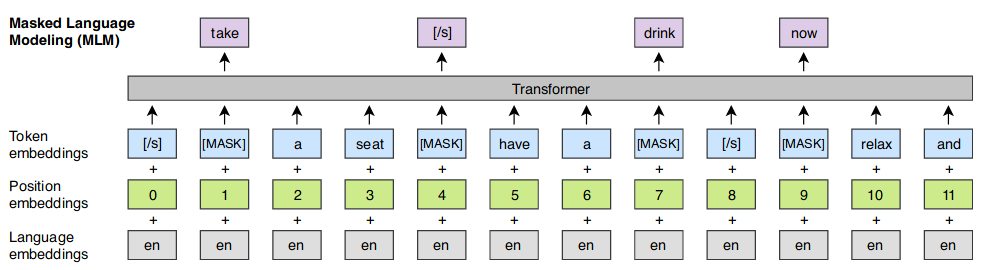
\includegraphics[scale=1.35]{img/xlm.png}
    \end{center}
\end{frame}

\begin{frame}
    \frametitle{XLM}
    \begin{center}
    	\begin{tabular}{l | l | l | l | l | l | l}
    	    \textbf{Model} & \textbf{Score} & \textbf{CoLA} & \textbf{SST2} & \textbf{MRPC} & \textbf{STS-B} & \textbf{QQP} \\
    	    \hline
    	    BERT & 80.5 & 60.5 & 94.9 & 89.3/85.4 & 87.6/86.5 & 72.1/89.3 \\
    	    XLM & 82.8 & 62.9 & 95.6 & 90.7/87.1 & 88.8/88.2 & 73.2/89.8 \\
    	\end{tabular}
    	
    	\begin{tabular}{l | l | l | l | l | l}
    	\textbf{MNLI\_m} & \textbf{MNLI\_mm} & \textbf{QNLI} & \textbf{RTE} & \textbf{WNLI} & \textbf{AX} \\
    	    \hline
    	86.7 & 85.9 & 92.7 & 70.1 & 65.1 & 39.6 \\
    	89.1 & 88.5 & 94.0 & 76.0 & 71.9 & 44.7 \\
    	\end{tabular}
    \end{center}
\end{frame}




% TransformerXL 
\section{TransformerXL}
\begin{frame}
    \frametitle{TransformerXL \cite{transformerxl}}
    \begin{itemize}
        \item June 2019
        \item Vanilla Transformer Language Models
        \begin{itemize}
            \item limited by a fixed-length context
            \item ignore all contextual information from previous segments (information never flow over segments)
        \end{itemize}
        \item TransformerXL
        \begin{itemize}
            \item "Recurrence" mechanism
            \item Relative Positional Encoding
        \end{itemize}
    \end{itemize}
\end{frame}

\begin{frame}
    \frametitle{Score}
    \begin{center}
        Vanilla Transformer: \\
        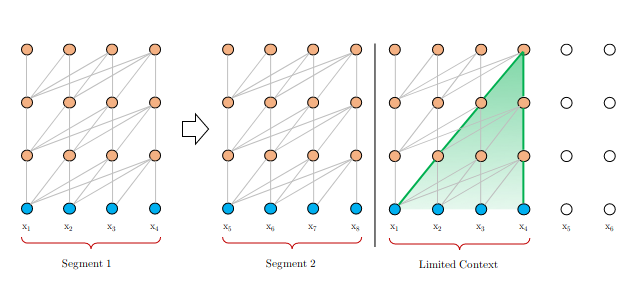
\includegraphics[scale=1.2]{img/transformerxl-train1.png} \\
        TransformerXL: \\
        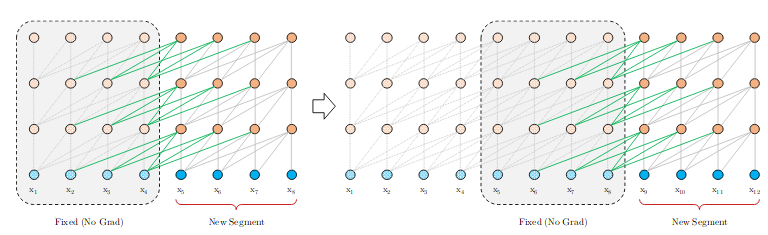
\includegraphics[scale=1.4]{img/transformerxl-train2.png}
    \end{center}
\end{frame}

\begin{frame}
    \frametitle{TransformerXL}
    \begin{itemize}
        \item "Recurrence" mechanism
        \begin{itemize}
            \item use fixed, cached segment (for each layer) from the previous segment
            \item use stop-gradient for caching
            \item different segments have the same positional encoding (an old segment is represented as [0, 1, 2, 3] and a new segment is processed as [0, 1, 2, 3, 0, 1, 2, 3] -- for the two segments)
        \end{itemize}
        \item Relative Positional Encoding
        \begin{itemize}
            \item encode relative positional information in the cached segment
            \item add content-dependent positional bias
        \end{itemize}
    \end{itemize}
\end{frame}

\begin{frame}
    \frametitle{Score}
    \begin{center}
    	\begin{tabular}{l | l | l | l}
    		\textbf{Method} & \textbf{enwiki8} & \textbf{text8} & \textbf{One Billion Word} \\
    		\hline
    		Previous best & 1.06 & 1.13 & 23.7 \\
    		\hline
    		TransformerXL & 0.99 & 1.08 & 21.8 \\
    	\end{tabular}
    	\begin{tabular}{l| l | l}
    	    \textbf{Method} & \textbf{WikiText-103} & \textbf{PTB} \\
    	    \hline
    	    Previous best & 20.5 & 55.5 \\
    		\hline
    	    TransformerXL & 18.4 & 54.5 \\
    	\end{tabular}
    \end{center}
\end{frame}



% Megatron-LM
\section{Megatron-LM}
\begin{frame}
    \frametitle{Megatron-LM \cite{megatronlm}}
    \begin{itemize}
        \item September 2019
        \item created by Nvidia
        \item support BERT and GPT-2 models training with the memory optimization
        \item use Wikipedia (without Wikitext-103 articles), CC-stories, RealNews, OpenWebtext -- 174 GB of text
        \item used 512 GPUs (Nvidia V100 32GB, trained over 9,2 days with 12 ZettaFLOPs)
        \item 480460 USD ($\sim$34 USD per hour -- one DGX-2) to train the GPT-2 model
    \end{itemize}
\end{frame}

\begin{frame}
    \frametitle{Parallelism}
    \begin{center}
        Speedup obtained for the 1.2 billion parameters model: \\
        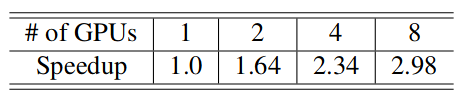
\includegraphics[scale=1.0]{img/megatron-lm-speedup.png} \\
        Hybrid Model and Data Parallelism: \\
        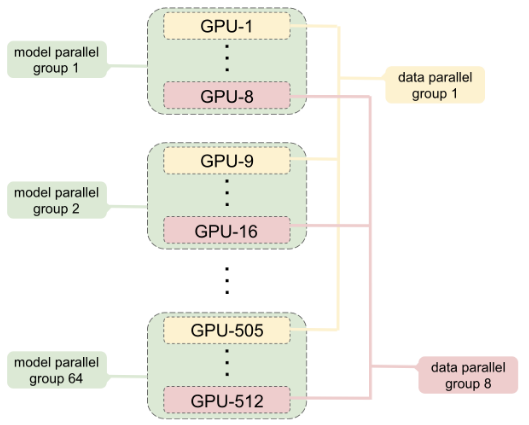
\includegraphics[scale=1.0]{img/megatron-lm-parallel.png}
    \end{center}
\end{frame}

\begin{frame}
    \frametitle{Score}
    \begin{center}
    	\begin{tabular}{l| l | l}
    	    \textbf{Model} & \textbf{Wikitext-103} & \textbf{LAMBADA} \\
    	     & Perplexity $\downarrow$ & Accuracy $\uparrow$ \\
    	    \hline
    	    355M & 19,31 & 45,16 \\
    	    2,5B & 12,76 & 61,73 \\
    	    8,3B & \textbf{10,81} & \textbf{66,51} \\
    		\hline
    	    SOTA & 16,43 & 63,24 \\
    	\end{tabular}
    \end{center}
\end{frame}



% XLNet
\section{XLNet}
\begin{frame}
    \frametitle{XLNet \cite{xlnet}}
    \begin{itemize}
        \item June 2019
        \item BERT + TransformerXL
        \item Permutation Language Modelling
        \item 245000 USD to train the XLNet model (to beat BERT on NLP tasks)
    \end{itemize}
\end{frame}

\begin{frame}
    \frametitle{autoregressive and autoencoding language modelling}
    \begin{itemize}
        \item autoregressive (AR) language modelling (classical)
        \begin{itemize}
            \item estimate the probability distribution of a text corpus
            \item trained to encode a uni-directional context (either forward or backward)
            \item is not effective at modelling deep bidirectional contexts
            \item downstream tasks often require bidirectional context information
        \end{itemize}
        \item autoencoding (AE) language modelling (like BERT)
        \begin{itemize}
            \item aims to reconstruct the original data from corrupted input ([MASK] token -- masked language model)
            \item density estimation is not part of the objective
        \end{itemize}
    \end{itemize}
\end{frame}

\begin{frame}
    \frametitle{Permutation Language Modelling}
    \begin{center}
        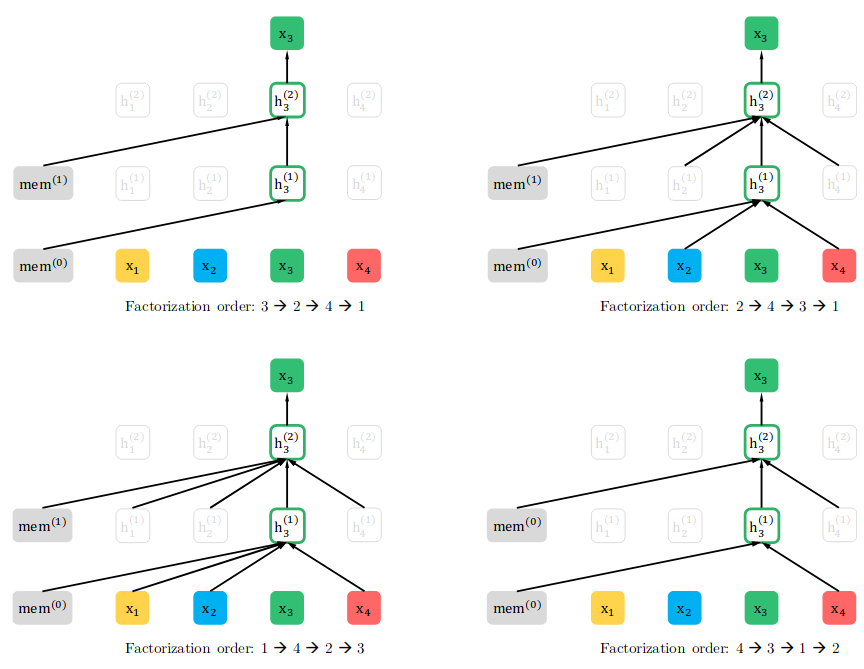
\includegraphics[scale=1.2]{img/XLNet-permutationlm.png}
    \end{center}
\end{frame}

\begin{frame}
    \frametitle{BERT vs XLNet}
    \begin{itemize}
        \item Sentence: [New, York, is, a, city]
        \item Select the two tokens: [New, York]
        \item Maximize: $log$ $p($New York $|$ is a city$)$
    \end{itemize}
    \begin{center}
    	\begin{tabular}{l| l | l}
    	    \textbf{Model} & \textbf{First prediction} & \textbf{Second prediction} \\
    	    \hline
    	    BERT & $log$ $p($New $|$ is a city$)$ & $log$ $p($York $|$ is a city$)$ \\
    	    XLNet & $log$ $p($New $|$ is a city$)$ & $log$ $p($York $|$ \textbf{New}, is a city$)$ \\
    	\end{tabular}
    \end{center}
\end{frame}

\begin{frame}
    \frametitle{Score}
    \begin{center}
        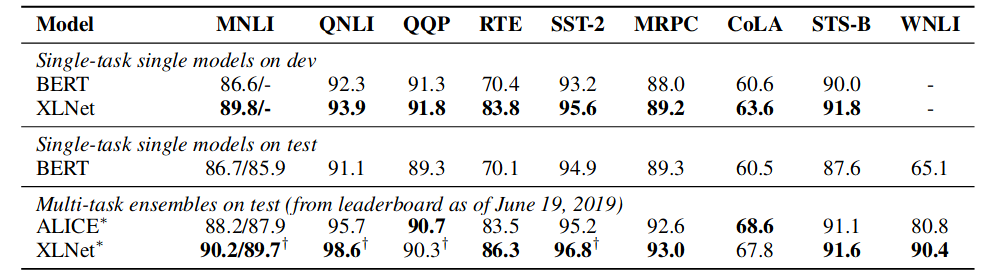
\includegraphics[scale=1.35]{img/XLNet-score.png}
    \end{center}
\end{frame}



% RoBERTa
\section{RoBERTa}
\begin{frame}
    \frametitle{RoBERTa -- \textbf{R}obustly \textbf{o}ptimized \textbf{BERT} \textbf{a}pproach \cite{roberta}}
    \begin{itemize}
        \item July 2019
        \item created by Facebook
        \item based on BERT
        \item more data (over 160GB) + more steps + larger batches (8K)
        \item no next sentence prediction
        \item dynamic masking instead of static
        \item larger byte level byte pair encoding vocabulary (50K units)
        \item used 1024 GPUs (Nvidia V100 32GB, trained over one day)
        \item 104448 USD ($\sim$34 USD per hour -- one DGX-2) to train the RoBERTa model
    \end{itemize}
\end{frame}

\begin{frame}
    \frametitle{Score}
    \begin{center}
        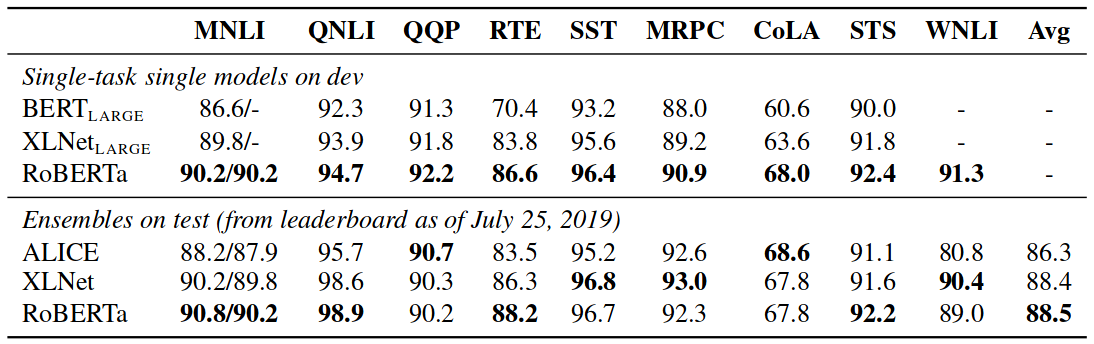
\includegraphics[scale=1.2]{img/RoBERTa-score.png}
    \end{center}
\end{frame}



% StructBERT
\section{StructBERT}
\begin{frame}
    \frametitle{StructBERT (ALICE -- Alibaba) \cite{structbert}}
    \begin{itemize}
        \item August 2019
        \item base on BERT
        \item Word Structural Objective -- ability to reconstruct the right order of certain number of intentionally shuffled word token
        \item Sentence Structural Objective -- extend the sentence prediction task by predicting both the next sentence and the previous sentence
        \item used 64 GPUs (Nvidia V100, trained over 38 hours/7 days)
        \item 8208-10336 USD ($\sim$27-34 USD per hour) to train base model and 36288-45696 USD to train huge model
    \end{itemize}
\end{frame}

\begin{frame}
    \frametitle{Word Structural Objective}
    \begin{center}
        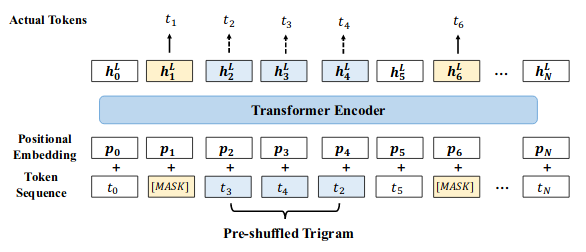
\includegraphics[scale=1.35]{img/StructBERT-wso.png}
    \end{center}
\end{frame}

\begin{frame}
    \frametitle{Sentence Structural Objective}
    \begin{center}
        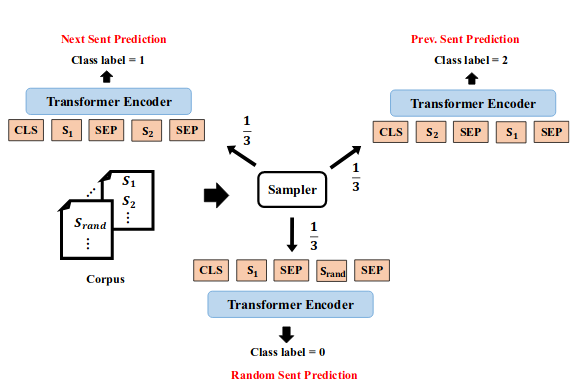
\includegraphics[scale=1.35]{img/StructBERT-sso.png}
    \end{center}
\end{frame}

\begin{frame}
    \frametitle{Score (old)}
    \begin{center}
        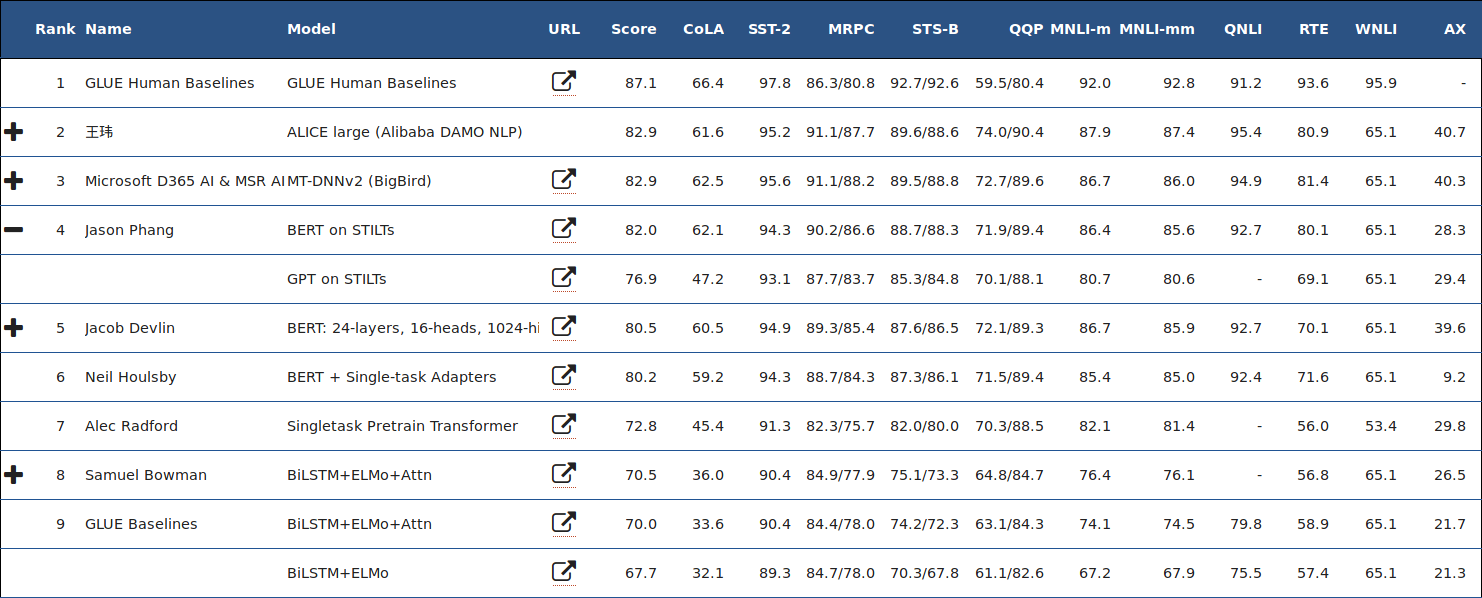
\includegraphics[scale=0.9]{img/glue_leaderboard_old.png}
    \end{center}
\end{frame}

\begin{frame}
    \frametitle{Score}
    \begin{center}
        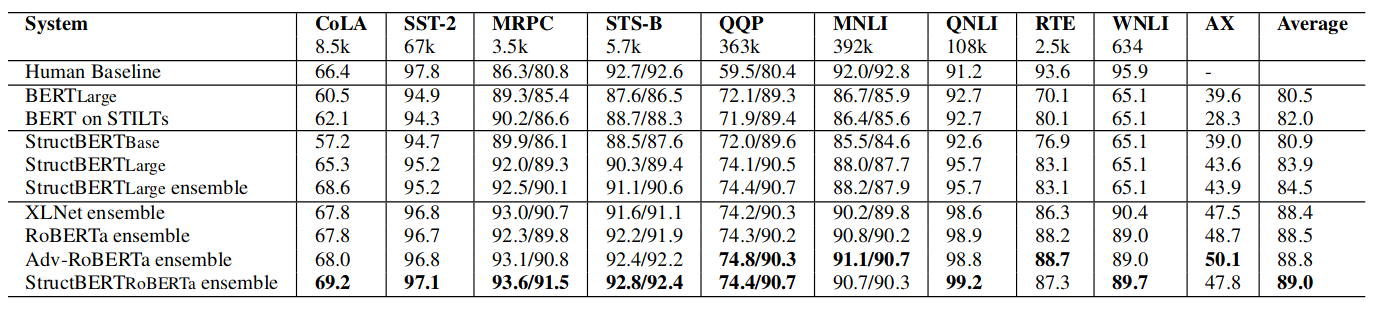
\includegraphics[scale=1.0]{img/StructBERT-score.png}
    \end{center}
\end{frame}



% ALBERT
\section{ALBERT}
\begin{frame}
    \frametitle{ALBERT -- A Lite BERT \cite{albert}}
    \begin{itemize}
        \item October 2019
        \item base on BERT
        \item factorized embedding parameterization (decomposing into two smaller matrices)
        \item use sentence-order prediction (SOP)
        \item cross-layer parameters sharing
        \begin{itemize}
        	\item share only attention parameters
        	\item share only FNN parameters
        	\item share attention and FNN parameters
        \end{itemize}
    \end{itemize}
\end{frame}

\begin{frame}
    \frametitle{NSP -- next sentence prediction\\SOP -- sentence-order prediction}
    \begin{center}
        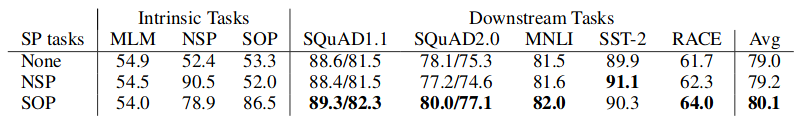
\includegraphics[scale=1.4]{img/albert-sop.png}
    \end{center}
\end{frame}

\begin{frame}
    \frametitle{BERT vs ALBERT}
    \begin{center}
        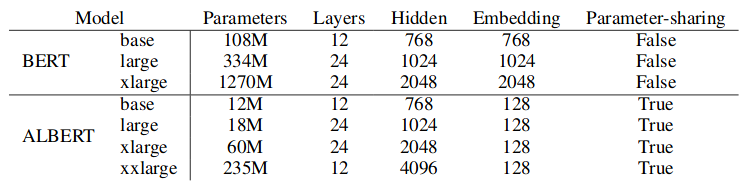
\includegraphics[scale=1.4]{img/albert-models.png} \\
        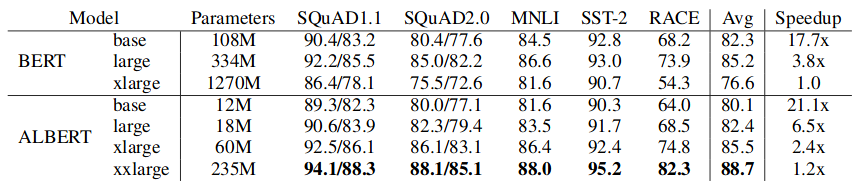
\includegraphics[scale=1.4]{img/albert-score-bert.png}
    \end{center}
\end{frame}

\begin{frame}
    \frametitle{Score}
    \begin{center}
        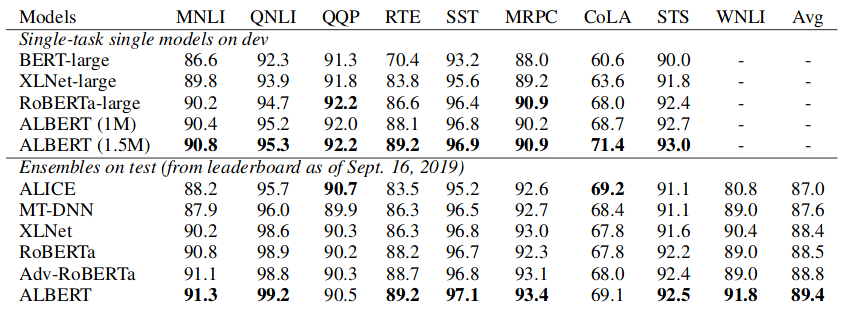
\includegraphics[scale=1.5]{img/albert-score.png}
    \end{center}
\end{frame}



% Other
\section{Other models}
\begin{frame}
    \frametitle{Other models}
    \begin{itemize}
        \item TinyBERT \cite{tidybert}
        \begin{itemize}
            \item September 2019
            \item transfer the knowledge of a large teacher network to a small student network
            \item 7,5 smaller, 9,4 faster, 28\% parameters of BERT
        \end{itemize}
        \item CTRL -- Conditional Transformer Language \cite{ctrl}
        \begin{itemize}
            \item September 2019
            \item use 140GB of text from a wide variety of domains
            \item large vocabulary of roughly 250k tokens
            \item control codes (to generate task-specific data)
            \item trained 2 weeks
        \end{itemize}
    \end{itemize}
\end{frame}



% T5
\section{T5}
\begin{frame}
    \frametitle{T5 -- Text-to-Text Transfer Transformer \cite{t5}}
    \begin{itemize}
        \item October 2019
        \item treat every NLP problem as a "text-to-text" problem (taking text as input and producing new text as output)
        \item based on Transformer (encoder and decoder)
        \item used "Colossal Clean Crawled Corpus" (called C4) -- about 750 GB of text (this is only extracted text from April 2019)
        \item for fine-tuning use all of the task as a single task by concatenating all of the datasets (with the special processing into input and output form)
        \item trained on 1024 TPU v3 (TPU v2 costs $\sim$768 USD per hour)
    \end{itemize}
\end{frame}

\begin{frame}
    \frametitle{Idea}
    \begin{center}
        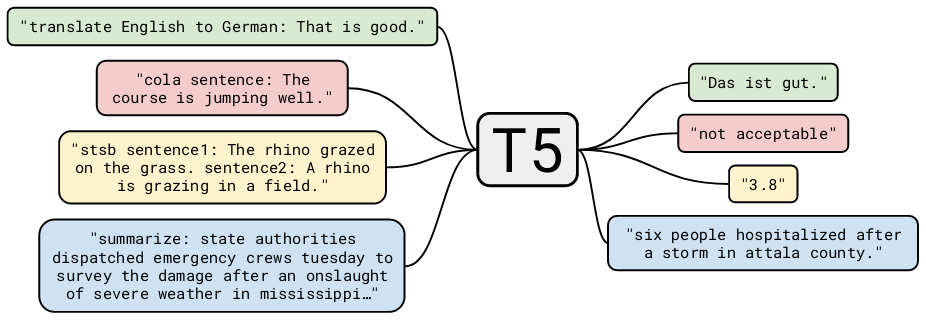
\includegraphics[scale=1.4]{img/t5-idea.png}
    \end{center}
\end{frame}

\begin{frame}
    \frametitle{Pre-training}
    \begin{center}
        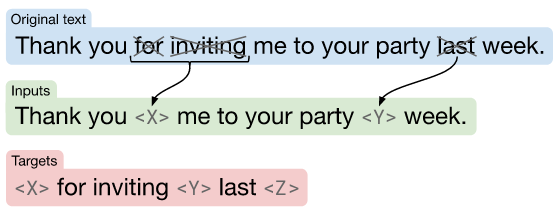
\includegraphics[scale=1.4]{img/t5-baseline-model.png}
    \end{center}
\end{frame}

\begin{frame}
    \frametitle{Score (GLUE)}
    \begin{center}
        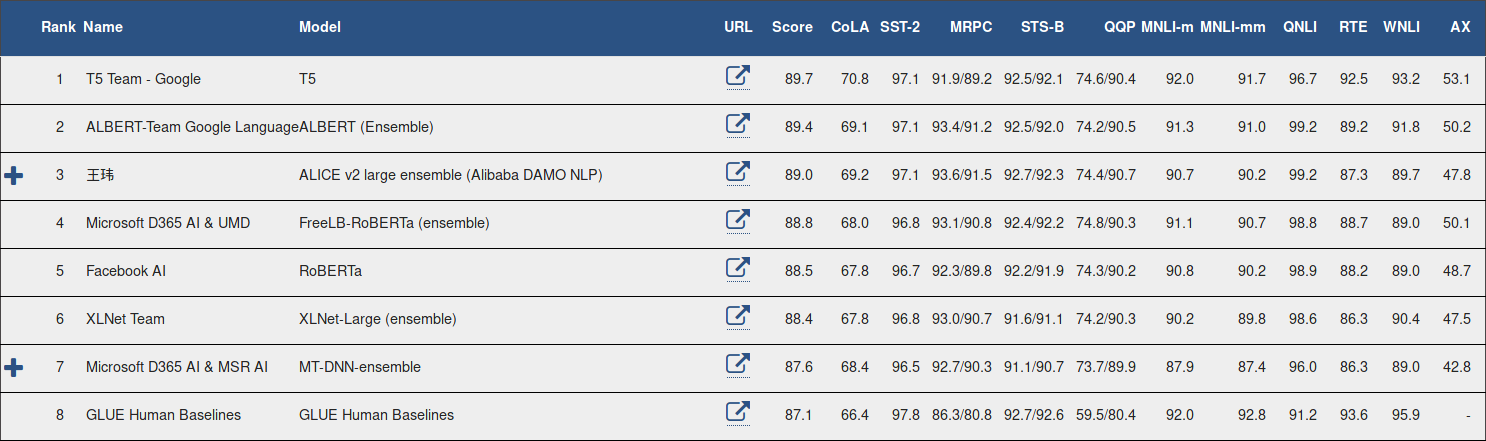
\includegraphics[scale=0.9]{img/glue_leaderboard.png}
    \end{center}

    \scriptsize
    \begin{tabular}{l| l | l | l | l | l | l}
    	& ALBERT & T5-Small & T5-Base & T5-Targe & T5-3B & T5-11B \\
    	\hline
    	Score & 89,4 & 77,4 & 82,7 & 86,4 & 88,5 & 89,7 \\
    \end{tabular}
\end{frame}

\begin{frame}
    \frametitle{Score (SuperGLUE)}
    \begin{center}
        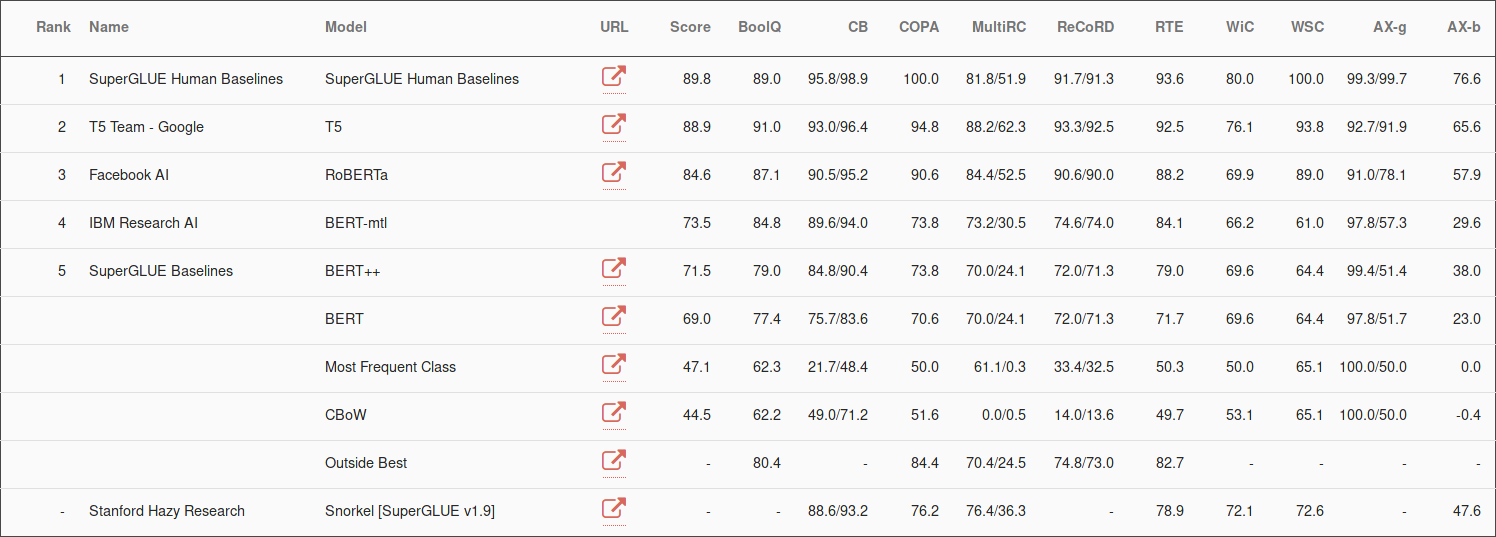
\includegraphics[scale=0.9]{img/super_glue_leaderboard.png}
    \end{center}
\end{frame}


% References
\section{References}
\begin{frame}[allowframebreaks,t]
    \tiny
    \frametitle{References}
    \bibliographystyle{ieeetr}
    \bibliography{language_model}
    %\nocite{*}
\end{frame}

\end{document}
